\documentclass[conference]{IEEEtran}
\IEEEoverridecommandlockouts
\usepackage{cite}
\usepackage{amsmath,amssymb,amsfonts}
\usepackage{algorithmic}
\usepackage{graphicx}
\usepackage{textcomp}
\usepackage{xcolor}
\usepackage{hyperref}
\usepackage{url}
\def\UrlBreaks{\do\A\do\B\do\C\do\D\do\E\do\F\do\G\do\H\do\I\do\J
\do\K\do\L\do\M\do\N\do\O\do\P\do\Q\do\R\do\S\do\T\do\U\do\V
\do\W\do\X\do\Y\do\Z\do\[\do\\\do\]\do\^\do\_\do\`\do\a\do\b
\do\c\do\d\do\e\do\f\do\g\do\h\do\i\do\j\do\k\do\l\do\m\do\n
\do\o\do\p\do\q\do\r\do\s\do\t\do\u\do\v\do\w\do\x\do\y\do\z
\do\.\do\@\do\\\do\/\do\!\do\_\do\|\do\;\do\>\do\]\do\)\do\,
\do\?\do\'\do+\do\=\do\#} 
\def\BibTeX{{\rm B\kern-.05em{\sc i\kern-.025em b}\kern-.08em
    T\kern-.1667em\lower.7ex\hbox{E}\kern-.125emX}}
\begin{document}

\title{High-Performance scRNA-seq Data Processing with Low-Redundancy Disk Access}

\author{\IEEEauthorblockN{Yu Liu}
\IEEEauthorblockA{\textit{School of Informatics} \\
\textit{Xiamen University}\\
Xiamen, China \\
liuyu123@stu.xmu.edu.cn}
\and
\IEEEauthorblockN{Mingxuan Gao}
\IEEEauthorblockA{\textit{School of Informatics} \\
\textit{Xiamen University}\\
Xiamen, China \\
mingxuangao@stu.xmu.edu.cn}
\and
\IEEEauthorblockN{Lixuan Tan}
\IEEEauthorblockA{\textit{School of Informatics} \\
\textit{Xiamen University}\\
Xiamen, China \\
tanlix@stu.xmu.edu.cn}
\and
\IEEEauthorblockN{Hongjin Liu}
\IEEEauthorblockA{\textit{School of Informatics} \\
\textit{Xiamen University}\\
Xiamen, China \\
liuhongjin@stu.xmu.edu.cn}
\and
\IEEEauthorblockN{Yating Lin}
\IEEEauthorblockA{\textit{School of Informatics} \\
\textit{Xiamen University}\\
Xiamen, China \\
linyating@stu.xmu.edu.cn}
\and
\IEEEauthorblockN{Wenxian Yang}
\IEEEauthorblockA{\textit{Aginome Scientific} \\
Xiamen, China \\
wx@aginome.com}
\and
\IEEEauthorblockN{Rongshan Yu*}
\IEEEauthorblockA{\textit{School of Informatics} \\
\textit{Xiamen University}\\
Xiamen, China \\
rsyu@xmu.edu.cn}
}

\maketitle

\begin{abstract}

High-throughput single-cell RNA sequencing (scRNA-seq) data processing pipelines integrate multiple modules to transform raw scRNA-seq data to gene expression matrices, including barcode processing, sequence quality control, genome alignment and transcript quantification.
With the rapid growth in data volume, the speed of scRNA-seq data processing pipeline has become a major bottleneck to large-scale scRNA-seq studies. 
%Here we introduce Falco, a cloud-based framework to enable paralellisation of existing RNA-seq processing pipelines using big data technologies of Apache Hadoop and Apache Spark for performing massively parallel analysis of large scale transcriptomic data. 
We present scSpark, a cloud computing based scRNA-seq data processing pipeline. 
% We combined Spark and our proposed functionalities to implement sequence quality control and transcript counting. 
%To reduce unnecessary disk access while reading FASTQ files and writing SAM files, we used the Java Native Interface (JNI) to deliver FASTQ Resilient Distributed Datasets (RDD), and retrieved genome mapping resul ts to SAM RDD. 
%Using two public scRNA-seq data sets and two popular RNA-seq alignment/feature quantification pipelines, we show that the same processing pipeline runs 2.6 – 145.4 times faster using Falco than running on a highly optimised single node analysis.
By leveraging Apache Spark's in-memory computing capability, scSpark significantly improves the processing speed of scRNA-seq data, and achieves 5\-20 times faster than the state-of-the-art processing pipelines under the same CPU core consumption.
In addition, thanks to Spark's inherent scalability in a cloud computing environment, scSpark can further reduce the processing time for a typical scRNA-seq dataset (e.g., 640 million reads) from hours to minutes when multiple computer nodes (e.g., 16) are used.  
Biological evaluation also confirmed that the results generated by scSpark are highly consistent with existing scRNA-seq data processing pipelines.
\end{abstract}

\begin{IEEEkeywords}
% Intermediate Data, Fast, Scalable
scRNA-seq data processing, Apache Spark, cloud computing
\end{IEEEkeywords}

\section{Introduction}
Single cell is the fundamental unit of a living organism.
Historically, RNA-seq has been widely used to study gene expression patterns in biological samples.
However, the resolution of bulk RNA-seq could only reach the average level of cell populations. 
With the development of single-cell sequencing technologies, scRNA-seq now allows transcript profiling of thousands of cells simultaneously in a single experiment, and has emerged as a powerful tool to identify and characterize cell types in complex and heterogeneous biological samples~\cite{Zhang2019ComparativeAO}.

%In order to demultiplex the reads for inidividual cells after sequencing~\cite{Tian2018scPipe}, two oligonucleotide barcodes, the cell barcode (CB) and the unique molecular identifier (UMI), have been introduced in single cell sequencing~\cite{Rosenberg2018SinglecellPO,Cao2017ComprehensiveSC}.  When using the CB, different barcode sequences are assigned to each cell for transcript source retrieval after sequencing, thus greatly improving the throughput and reducing the cost of scRNA-seq~\cite{Macosko2015HighlyPG,Klein2015DropletBF}. UMIs are random oligonucleotide barcodes used in single cell sequencing to distinguish redundant transcripts generated from PCR amplification~\cite{Kivioja2012Counting,Camara2017Methods,Smith2017UMItools}. 

To enable efficient scRNA-seq data processing, various pipelines have been developed.
A fully-functioned scRNA-seq data processing pipeline typically implements multiple modules including the unique molecular identifier (UMI) barcode~\cite{Smith2017UMItools} processing, sequence quality control (QC)~\cite{schmieder2011quality}, genome alignment~\cite{Dobin2013STAR,Kim2015HISAT} and transcript quantification~\cite{Parekh2018zUMIs} to convert raw scRNA-seq data into a gene expression matrix for further downstream analysis. 
%First, the barcodes are extracted from a pre-designed nucleotide site for different scRNA-seq protocols. In QC, the FASTQ reads with low quality nucleotides are filtered based on user-defined thresholds.  Subsequently, the remaining FASTQ reads are mapped to the reference genome using a splice-aware aligner, such as STAR~\cite{Dobin2013STAR} and HISAT2~\cite{Kim2015HISAT}. Finally, the reads are assigned to genes and the count matrices for UMIs are generated~\cite{Parekh2018zUMIs}. 
Among all the scRNA-seq data processing pipelines, the most influential studies probably include CellRanger~\cite{Zheng2017Massively}, UMI-tools~\cite{Smith2017UMItools}, and STARsolo~\cite{Blibaum2019STARsolo}, etc. 
CellRanger is a highly integrated data processing software tool tailored by 10X Genomics for scRNA-seq data analysis.
It is most suitable for processing large datasets on high performance workstations~\cite{Gao2020Comparison}. 
UMI-tools is a comprehensive scRNA-seq data processing suite with the directional barcode collapse algorithm integrated that considerably promotes the transcript quantification accuracy.
STARsolo is a recently developed pipeline extended from the genome aligner STAR to adapt to single cell applications. 
%However, these scRNA-seq data processing pipelines lack the scalability to meet the computational demand from the large volume of scRNA-seq data from increasing numbers of single cell studies. 

In the big biological data era, large amount of data can be produced in a short time with low cost. 
The computational demand from the large volume of scRNA-seq data from increasing numbers of single cell studies is becoming tremendous and surpassed the capabilities of these traditional bioinformatics tools. 
The cloud computing environment is a distributed system with extremely scalable computation capabilities, and allows users to run applications and services on a distributed network using a virtualized system. 
Recently, big data frameworks such as Apache Hadoop (\url{https://hadoop.apache.org}) and Apache Spark (\url{https://spark.apache.org}) have been used to speed up the data processing for next generation sequencing (NGS) data. 
SparkBWA~\cite{Abun2016SparkBWA} exploits the capabilities of Spark to boost the performance of a most widely used NGS data aligner, the Burrows-Wheeler Aligner (BWA). 
GPF~\cite{Li2018Highperformance} is a fast in-memory computing framework designed using the Spark framework for implementing NGS data processing pipelines in cloud computing environment. 
Following the success of cloud-based implementations of NGS data processing pipelines, Falco~\cite{Yang2017Falco} concatenates the genome aligner and transcript quantification software tools using Spark for scRNA-seq data preprocessing.
Although Falco improves the performance of scRNA-seq data processing when a distributed computing environment is available, it does not support UMI barcode processing. Hence, it is incompatible with the widely-used high-throughput scRNA-seq protocols such as 10X Genomics, Drop-seq and Microwell-seq. In addition, it does not leverage the in-memory computing capability of Spark to reduce the disk read and write operations of intermediate data processing steps. Therefore, further performance speedup could be expected. 

To meet the growing computational demand of processing large-scale scRNA-seq data, we present scSpark, an in-cloud and in-memory computing scRNA-seq data processing pipeline with high efficiency and scalability. 
More specifically, by implementing and integrating multiple procedures of a standard scRNA-seq data processing pipeline with the aid of in-memory computing schema of Spark, scSpark eliminates the need for laborious disk read/write operations associated with traditional bioinformatics tools. 
As a result, scSpark is able to improve the speed for scRNA-seq data processing by more than 10 folds compared with other state-of-the-art software tools under the same CPU core consumption. In addition, by harnessing the merit of the parallel computing capability of Spark engine, scSpark further enables users to distribute their scRNA-seq data processing workloads to multiple computational nodes, thus dramatically increases their processing throughput of scRNA-seq data for large-scale studies. 
scSpark is freely available at \url{https://github.com/xmuyulab/spark-scRNASeq-Analysis.git}.
%After Introduction, we provides method to implement scSpark. Subsequenctly, we evaluates scSpark on a 256 (16*16) cores compute cluster and analyzes scSpark's performance and scalability. Finally, we conlude ..  concluding in the end.

% GPF is freely available: https://github.com/fhyxz/GPF.git. This paper is organized as follows: Section 2 provides background information on genomic analytics pipelines. Section 3 ex- plains the APIs of the GPF, and Section 4 describes the exe- cution engine of GPF. Section 5 evaluates our solution on a 2048 cores compute cluster and analyzes the most important factors to the performance of our GPF. Finally, we discuss related work in Section 6 before concluding in Section 7.

\section{Method}
\subsection{Overview}
Apache Spark is a lightning fast, in-memory data processing engine.
It distributes data in a file system across the cluster and process that data in parallel. 
In Spark, an Resilient Distributed Dataset (RDD)~\cite{Zaharia2012Resilient} is a read-only collection of data items that can be divided into logical partitions and distributed over a cluster of nodes for parallel computing. 
By using RDDs, Apache Spark keeps things in memory and allows to cache data in memory, hence reduces time for disk I/O.
%
We developed scSpark on top of the Spark framework~\cite{zaharia2010spark} to leverage its two major features for fast scRNA-seq data processing, i.e., parallel computing and in-memory computing. 
On the other hand, the functional workflow of scSpark follows closely with that of UMI-tools.
Briefly, our scRNA-seq data processing pipeline consists of three major steps, data loading with whitelist control, alignment of extracted reads to a reference genome, and transcript quantification. 
%Next we explain the design principle and implementation details of each step of scSpark. 

\subsection{Data loading with whitelist control}
\iffalse
\begin{figure}
	\centering
		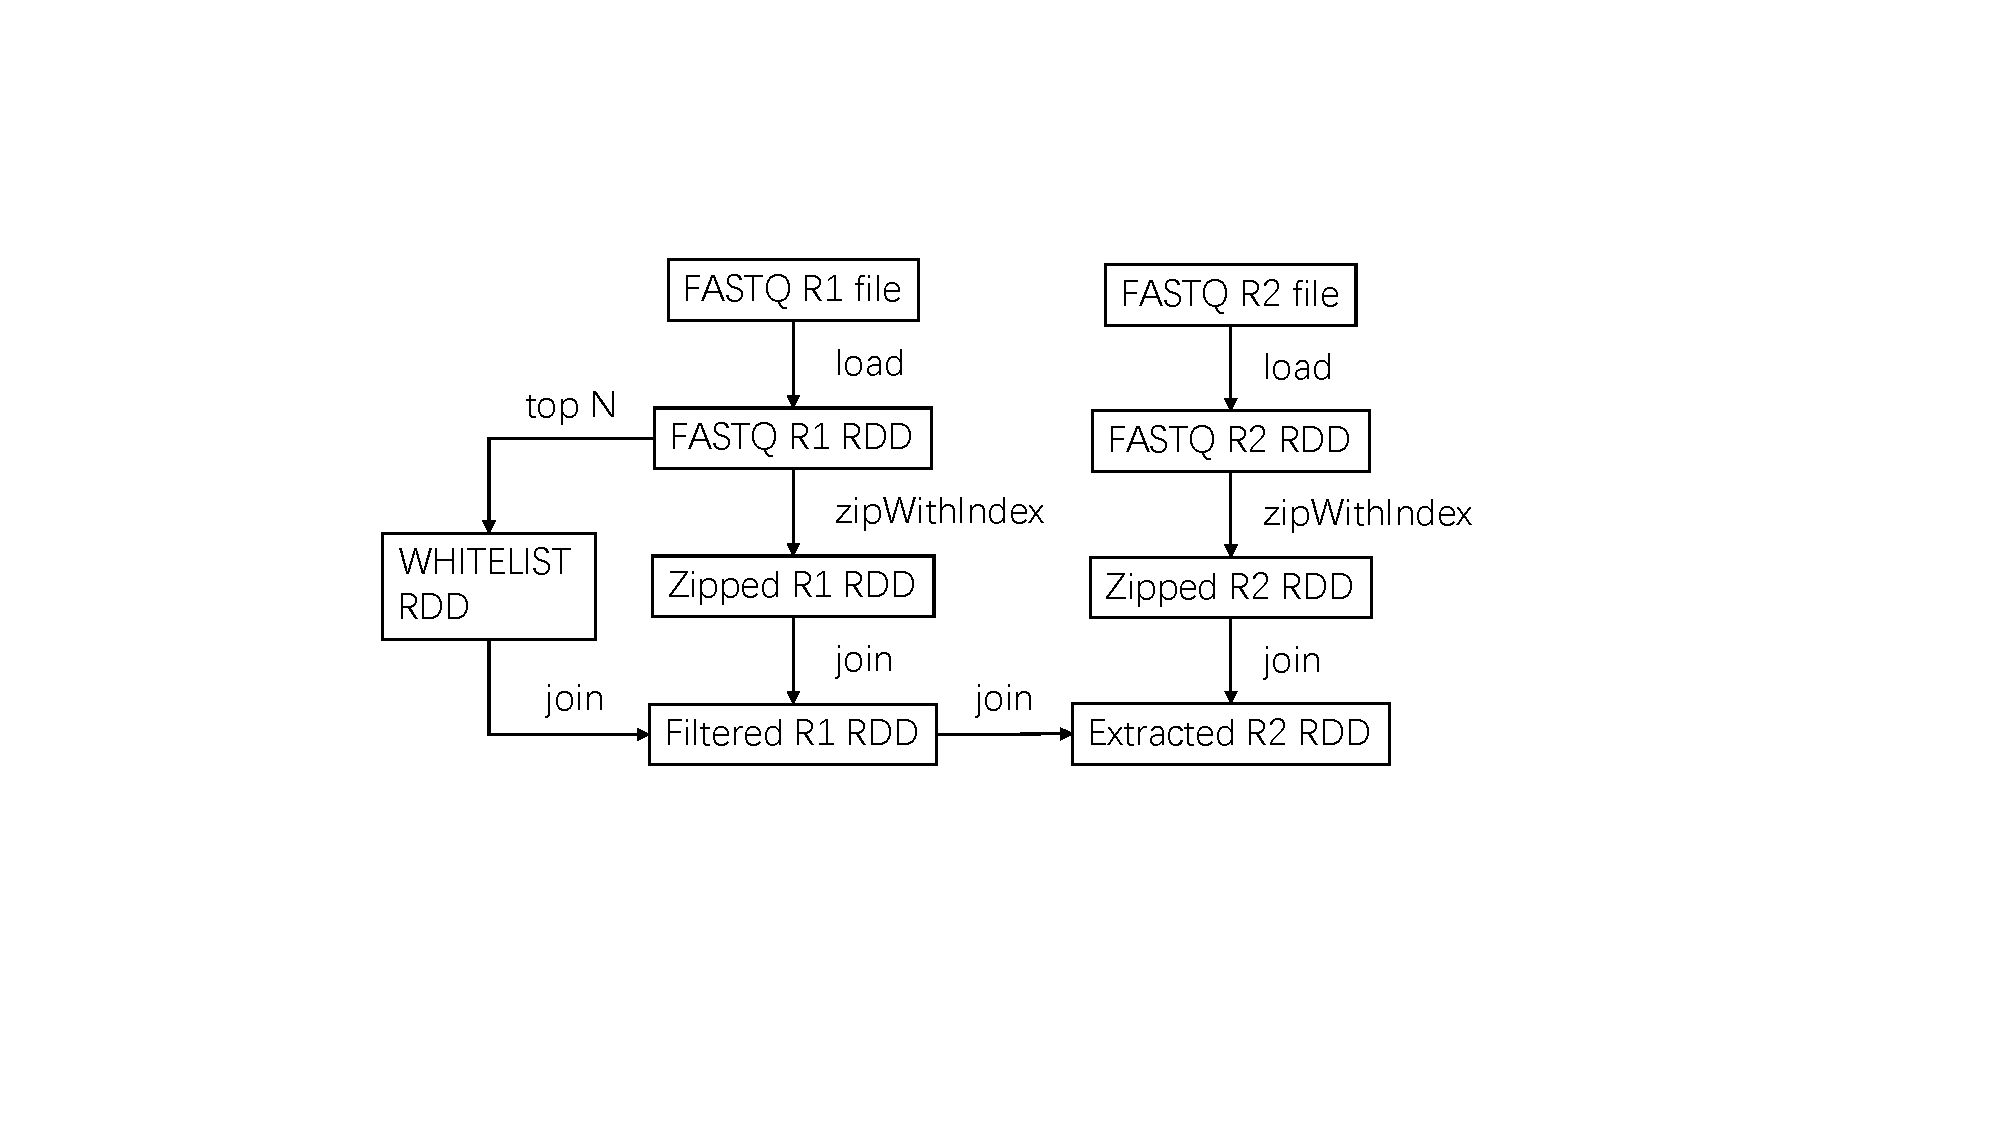
\includegraphics[width=0.35\textwidth]{figure1.pdf}
		\caption{Data loading with whitelist control.} \label{fig1}
	\end{figure}	
\fi

To construct RDD that contains the scRNA-seq reads for subsequent parallel in-memory processing, e.g., alignment, the following procedures are used (Fig.~\ref{fig1}).
First, we load each scRNA-seq read in FASTQ format~\cite{cock2010sanger} into one RDD (FASTQ RDD) using Hadoop-BAM~\cite{hadoopBAM}.
scSpark extracts cell barcode from the first read in a read-pair, which is then used as the key to index the UMI and transcript sequence from the read-pair.
Once the RDDs are constructed, we use the \textit{reduceBy} function of Spark to identify the highest-occurrent cell barcodes in the scRNA-seq dataset with user-defined threshold to create the whitelist~\cite{guo2018bioinformatics}, which are used to select valid reads for further processing. 

\subsection{Parallel genome alignment}
\begin{figure*}
\centering
	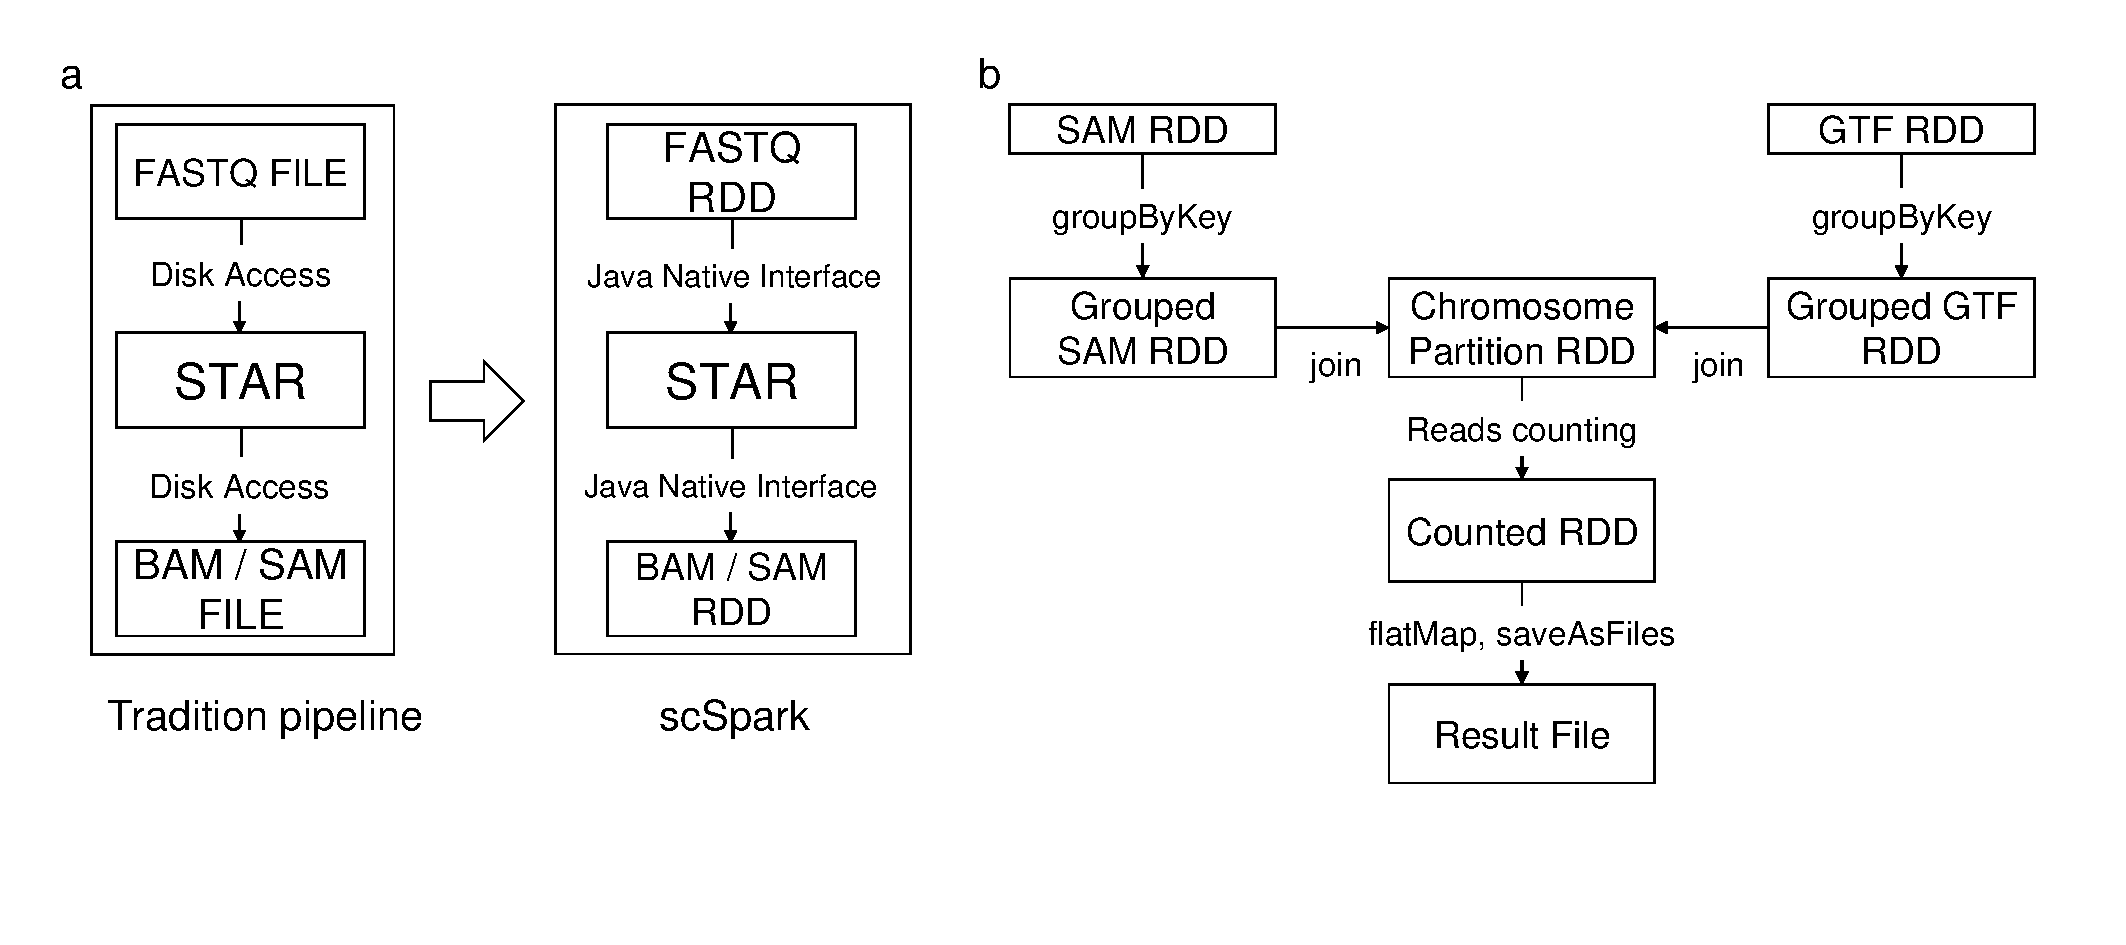
\includegraphics[width=0.9\textwidth]{fig2-3.pdf}
	\caption{Using JNI and RDD to integrate the STAR aligner in scSpark.} \label{fig1}
\end{figure*}

% ref: Parallelized Aligner: Thanks to the nature of embarrassing parallelism in terms of partitioning input data, raw reads can be mapped to the reference genome independently of one another in theory.
% ref: As shown in Figure 2, Aligner splits reads in FASTQ file into N sets in smaller files (FASTQ 1, FASTQ 2, FASTQ 3 ... FASTQ N), then align them to reference genome using the alignment component BWA (which is configurable for multithreading execution).
% ref: The final alignment results are stored in multiple SAM files.

As in CellRanger, UMI-tools and STARsolo, we also adopt STAR as the aligner in scSpark.
The conventional STAR alignment procedure loads raw reads from FASTQ files and write alignment results to Sequence Aligment/Map (SAM)~\cite{li2009sequence} files, requiring extensive disk access which consumes a significant amount of time.
Instead, in scSpark, we use the Java Native Interface (JNI) 
%~(\url{https://docs.oracle.com/javase/8/docs/technotes/guides/jni/}) 
to directly feed FASTQ RDD to STAR, and further transfer the results output from STAR to the SAM RDD after alignment (Fig.~\ref{fig1}.a). 
In such way, the alignment process is performed in an in-memory computing manner without any disk access. 

To balance the workloads across different nodes for parallel processing, we use the Spark function \textit{repartition} before alignment to split FASTQ RDDs into \textit{N} subsets where \textit{N} denotes the number of nodes available in the cluster. After data loading and partitioning, the STAR alignment is performed in parallel on all computational nodes, resulting in a SAM RDD which is used as input to the next module. 

\subsection{Transcript quantification}
% \begin{figure}
% \centering
% 	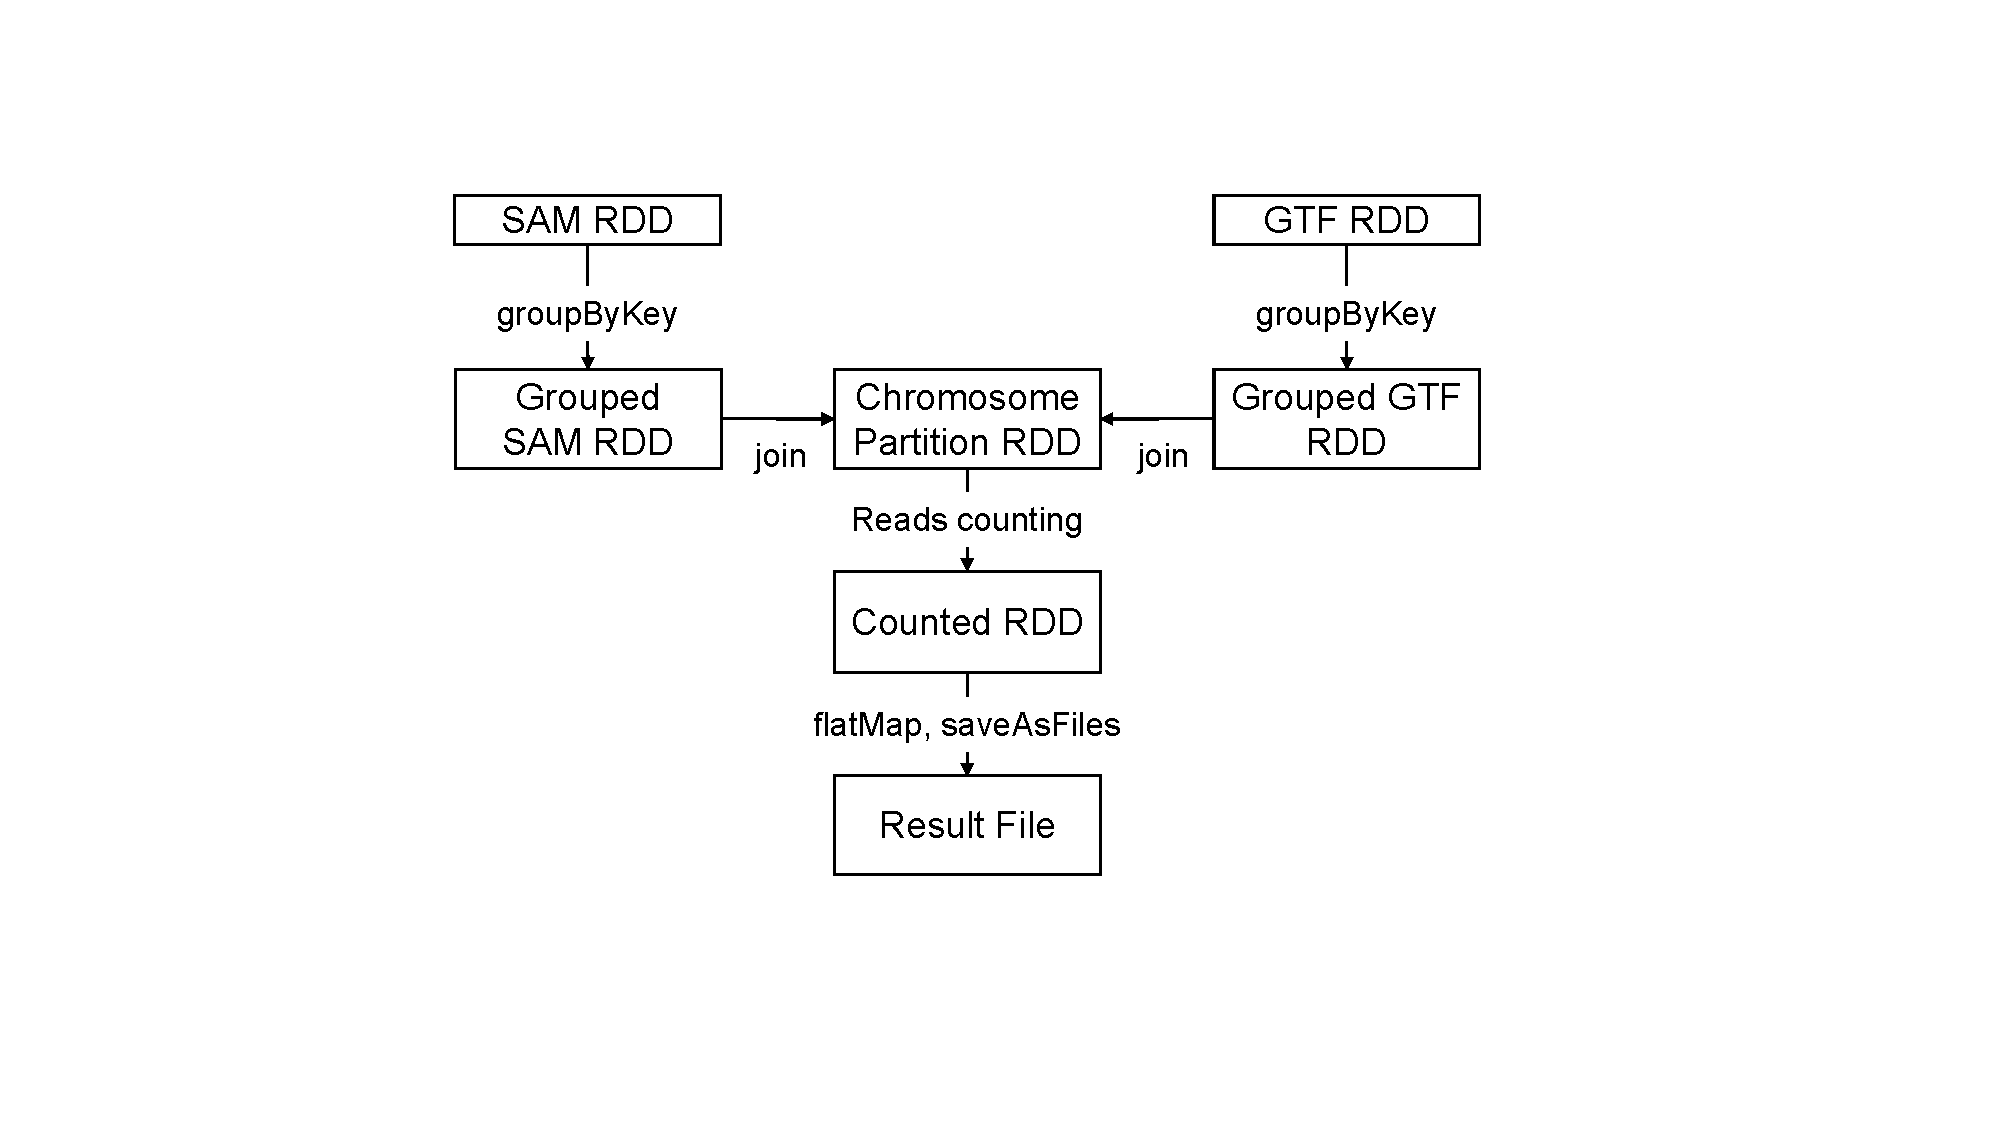
\includegraphics[width=0.45\textwidth]{figure3.pdf}
% 	\caption{An overview of Spark version count.} \label{fig3}
% \end{figure}

% ref: The execution engine of our GPF is designed in such manner that it builds the dependencies among processes according to the references among different resources.
% ref: The algorithm 1 presents a pseudo-code of the DAG analysis.
% ref: For example, when the output of Process A uses the same ref- erence as the input of Process B, B is dependent on A.
% ref: If Process is treated as a node and the dependency is as a directed edge from one node to another, the entire pipeline can be transformed into a DAG.
% ref: The engine then performs a topology sort on the DAG to generate a proper execution order.
% ref: It should be noted that the DAG may not be a connected graph.
% ref: Thus, it is necessary to iterate through the topology until all processes have been executed.
For transcript quantification, we first use the \textit{textFile} function in Spark to load the gene transfer format (GTF) file into memory as GTF RDDs (Fig.~\ref{fig1}.b). 
After alignment, all the SAM RDDs and GTF RDDs were grouped by chromosome into Grouped SAM RDDs and Grouped GTF RDDs respectively for parallel processing. 
The gene names are then assigned to each aligned read using the \textit{join} function. 
In scSpark, we reimplemented the directional algorithm designed by UMI-tools for transcript quantification using \textit{flatMap}. 
Finally, the resulting expression matrix is written to disk for further downstream analysis.
%The transcript quantification step of scSpark is designed in three substeps including loading gene transfer format (GTF)~\cite{breese2013ngsutils} file, using GTF to find gene's cell name, qualitfy each gene's quantity.
%Due to each GTF format's line represents one record, scSpark can easily transfer GTF format file to GTF RDD by using \textit{textFile}.

%After GTF RDD generated, as Fig.~\ref{fig3} shown, scSpark uses \textit{map} to set feature as SAM RDD and GTF RDD's key.
%ScSpark then uses \textit{groupByKey} to gather SAM RDD and GTF RDD by their key and conjunction SAM RDD and GTF RDD when they have same key.
%After that, scSpark could get Wait Count RDD which structure is like \textit{(Feature, SAM record, GTF record)}.

%Then scSpark performs a \textit{flatMap} on each feature, iterate through SAM record to matching GTF record and count in this substep's end.
%In this step end, scSpark use \textit{saveAsTextFile} can easily get result of scSpark for further downstream analysis. 

\section{Results}

\subsection{Experiment design}
The performance in processing speed of scSpark is compared with CellRanger, UMI-tools and STARsolo. 
We used Apache Spark (version 2.1.0) as scSpark's in-memory computing environment. 
Three scRNA-seq datasets containing peripheral blood mononuclear cells (PBMCs) from three different species, namely human, rat and monkey, generated by 10X Genomics platform were used in our experiments. 
In total, there are approximately 640 million, 289 million and 262 million reads in the raw data of the PBMC\_human, PBMC\_rat and PBMC\_monkey datasets, respectively. 
In all the experiments, we run all the four pipelines with exactly the same cell number and barcode pattern arguments. Pre-tests were performed to ensure sufficient memory for each pipeline.

% We evaluated the performance of scSpark with three state\-of\-the\-art pipelines including UMI-tools, CellRanger and STARsolo in terms of the efficiency, scalability and biological analysis accuracy.
% ref: To identify whether scale-out beyond 2048 cores is feasible, we systematically identified the potential performance bottlenecks of our GPF.
To identify whether scSpark get better performance than three state-of-the-art pipelines in same CPU cores number condition,
we compared scSpark's performance on a cluster with 64 (16$\times$4) CPU cores with three pipelines' performance on a workstation with 64 CPU cores.
%In this experiment, we used \textit{runThreadN} parameter to restrict STAR and STAR-solo occupy CPU cores number and used \textit{localcores} parameter to restrict CellRanger occupy CPU cores number.
In this experiment, the number of CPU cores used was configured using the \textit{runThreadN} parameter for STAR and STAR-solo, and using the \textit{localcores} parameter for CellRanger. 
Except align step, UMI-tools doesn't have parameter to specify pipeline will occupy how much CPU cores, so we tested it in a 64 CPU cores workstation. 
To test improvement in scSpark's performance as a result of improving each substep's performance,
we meatured UMI-tools and scSpark each substep's process time to prove scSpark get improve in any single substep.

Furthermore, to identify wherther scSpark's scalability is better than three tradition pipelines, 
we meatured each tradition pipelines' speedup by considering 16 CPU cores execution as a baseline.
And we used \textit{SPARK\_EXECUTOR\_CORES} parameter to restrict Spark cluster's CPU cores number, and meatured scSpark's speedup by considering 16 CPU cores execution as a baseline.
Particularly, we meatured STAR mapping's speedup by considering 16 CPU cores execution as a baseline and meatured scSpark mapping's speedup by considering 16 CPU cores execution as a baseline.

ScSpark is developed based on UMI-tools. 
And UMI-tools accuracy was fully verified. 
This section we used the gene expression matrix that was obtained by scSpark and UMI-tools under the same dataset to perform downstream analysis of scRNA-seq data. 
And then we compared two tools transcript analysis's result and cell cluster analysis's result to verify the correlation between scSpark and UMI-tools. 
Under hgmm-10k-v3 dataset, we used scSpark and UMI-tools to get gene express matrix, compared two tools' result, and computed their correlation.


\subsection{Efficiency evaluation}

\begin{table}
	\centering
	\caption{Comparison of processing time (seconds) of four pipelines.}\label{tab1}
	\begin{tabular}{l | l | l | l }
		\hline
		 & PBMC\_human & PBMC\_rat & PBMC\_monkey \\ 
		\hline
		UMI-tools & 7284 & 7259 & 7809 \\
		CellRanger & 2225 & 1999 & 1891 \\
		STARsolo & 1987 & 1854 & 2357 \\
		\textbf{scSpark} & \textbf{355} & \textbf{326} & \textbf{391} \\
		\hline
	\end{tabular}
\end{table}

We first evaluated the total time comsumption for different pipelines processing the same dataset with the same numbers of CPUs. 
For UMI-tools, CellRanger, and STARsolo, we used all 64 cores of a single workstation. 
For scSpark, we used a cluster of 4 computing nodes, where each node has 16 CPU cores. 
Results show that scSpark achieves substantially higher processing speed, which is nearly 20-fold faster than UMI-tools and about 5-fold faster than CellRanger and STARsolo (Table~\ref{tab1}). 
We also recorded the processing time for three individual modules of the pipelines, i.e., barcode extraction and sequence QC, genome alignment, and transcript quantification, to have a more detailed understanding of the performance gain. 
As scSpark is built based on UMI-tools, the breakdown comparison was only between UMI-tools and scSpark, to demonstrate the performance gain brought by distributed and in-memory computing. Compared with UMI-tools, scSpark had significantly shorter processing time in all three steps (Fig.~\ref{fig4}). It is noteworthy that scSpark achieved a processsing speed of approximately 50-fold  faster than UMI\-tools for the barcode extraction and sequence QC step, which turned out to be the dominant factor of the performance promotion brought by scSpark. This result reflects that distributed reading of FASTQ reads from disk and totally removal of re-writing extracted FASTQ reads back to disk that are both performed in scSpark can dramatically reduce the time consumption of scRNA-seq data processing pipelines. 

\iffalse
To illustrate the main source of the significant improvement brought by scSpark, we also compared the efficiency of three individual steps of the pipeline between scSpark and UMI-tools. 
%Table~\ref{tab1} gives a summary of scSpark's performance and compares with tradition pipeline's performance.
%We can see scSpark's speed is much quicker than any tradition pipelines in same CPU cores environment in three datasets.
\fi

\begin{figure*}
	\centering
	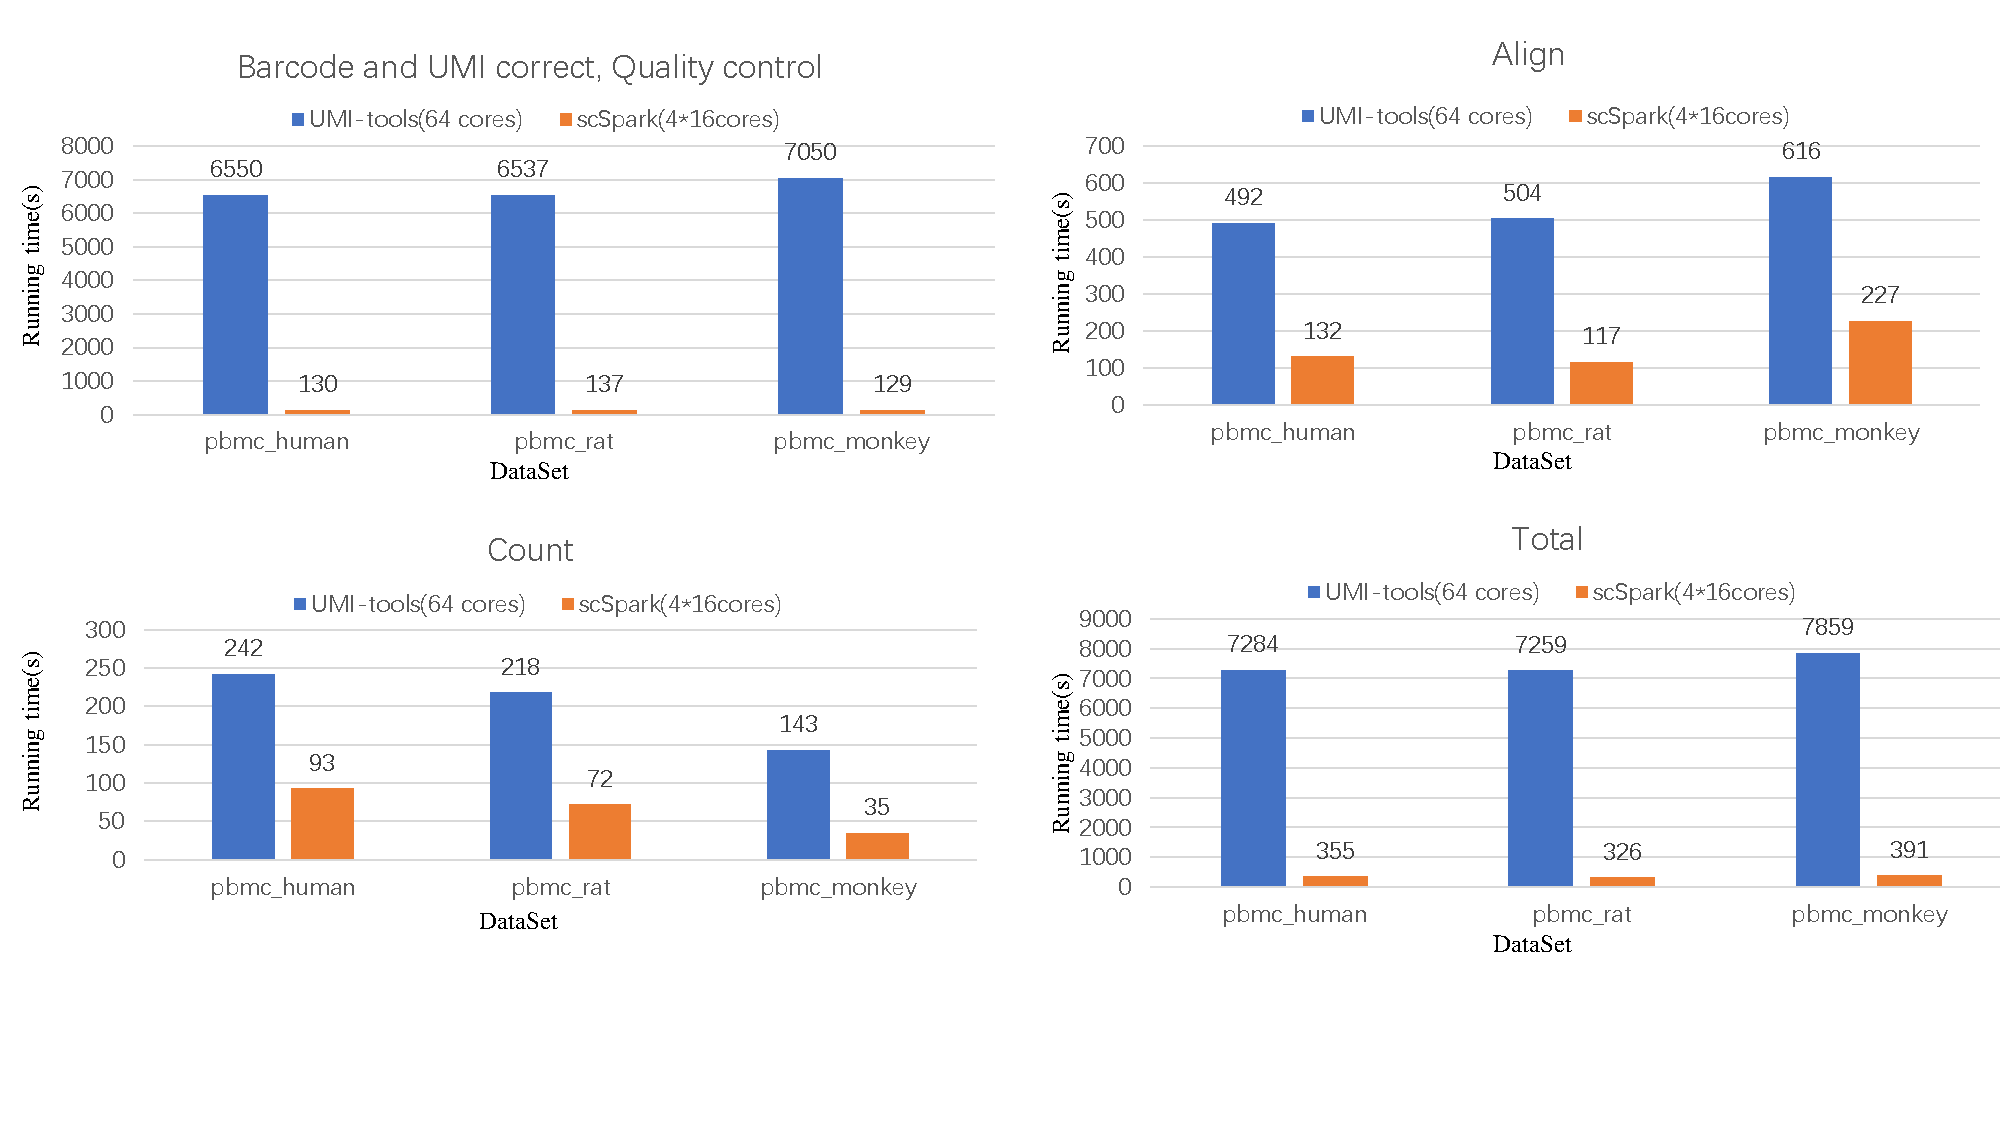
\includegraphics[width=0.9\textwidth]{fig4.pdf}
	\caption{Comparison of UMI\-tools and scSpark's first step.} \label{fig4}
\end{figure*}


\iffalse
After that we recorded each step's process time to find the reason of scSpark's speed improvement.
As table~\ref{fig4} shown, scSpark is much faster than the UMI-tools in any single step.
Contrast with UMI-tools, scSpark gets great improve in first two steps, cell barcode and UMI correct and quality control.
This step's improve comes from scSpark's in-memory trait which can reduce disk access times.
And scSpark can take advantage of Spark's high concurrency feature when UMI-tools processed record with single thread.

After that, scSpark use in-memory FASTQ RDD and SAM RDD to replace tradition pipeline's disk access. 
Although scSpark and UMI-tools's align step both based on STAR, scSpark can get great improve in same CPU cores condition.
Except reduce redundancy disk access, scSpark processes multi STAR program across Spark cluster in the same time also can improve scSpark's mapping speed.

After align step, we grouped SAM RDD and GTF RDD by cell and concurrency processed each group in each CPU cores.
Due to each cell's record number imbalance, scSpark's count step has a little data skew problem which causes count step's processing time influenced by dataset.
This way also gets great improve compare with UMI-tools.
\fi

\subsection{Evaluation of scalability} 
Contrast with tradition pipelines, scSpark not only can perform well in same CPU cores but also scSpark can scala out to improve process speed.
\begin{figure}
	\centering
	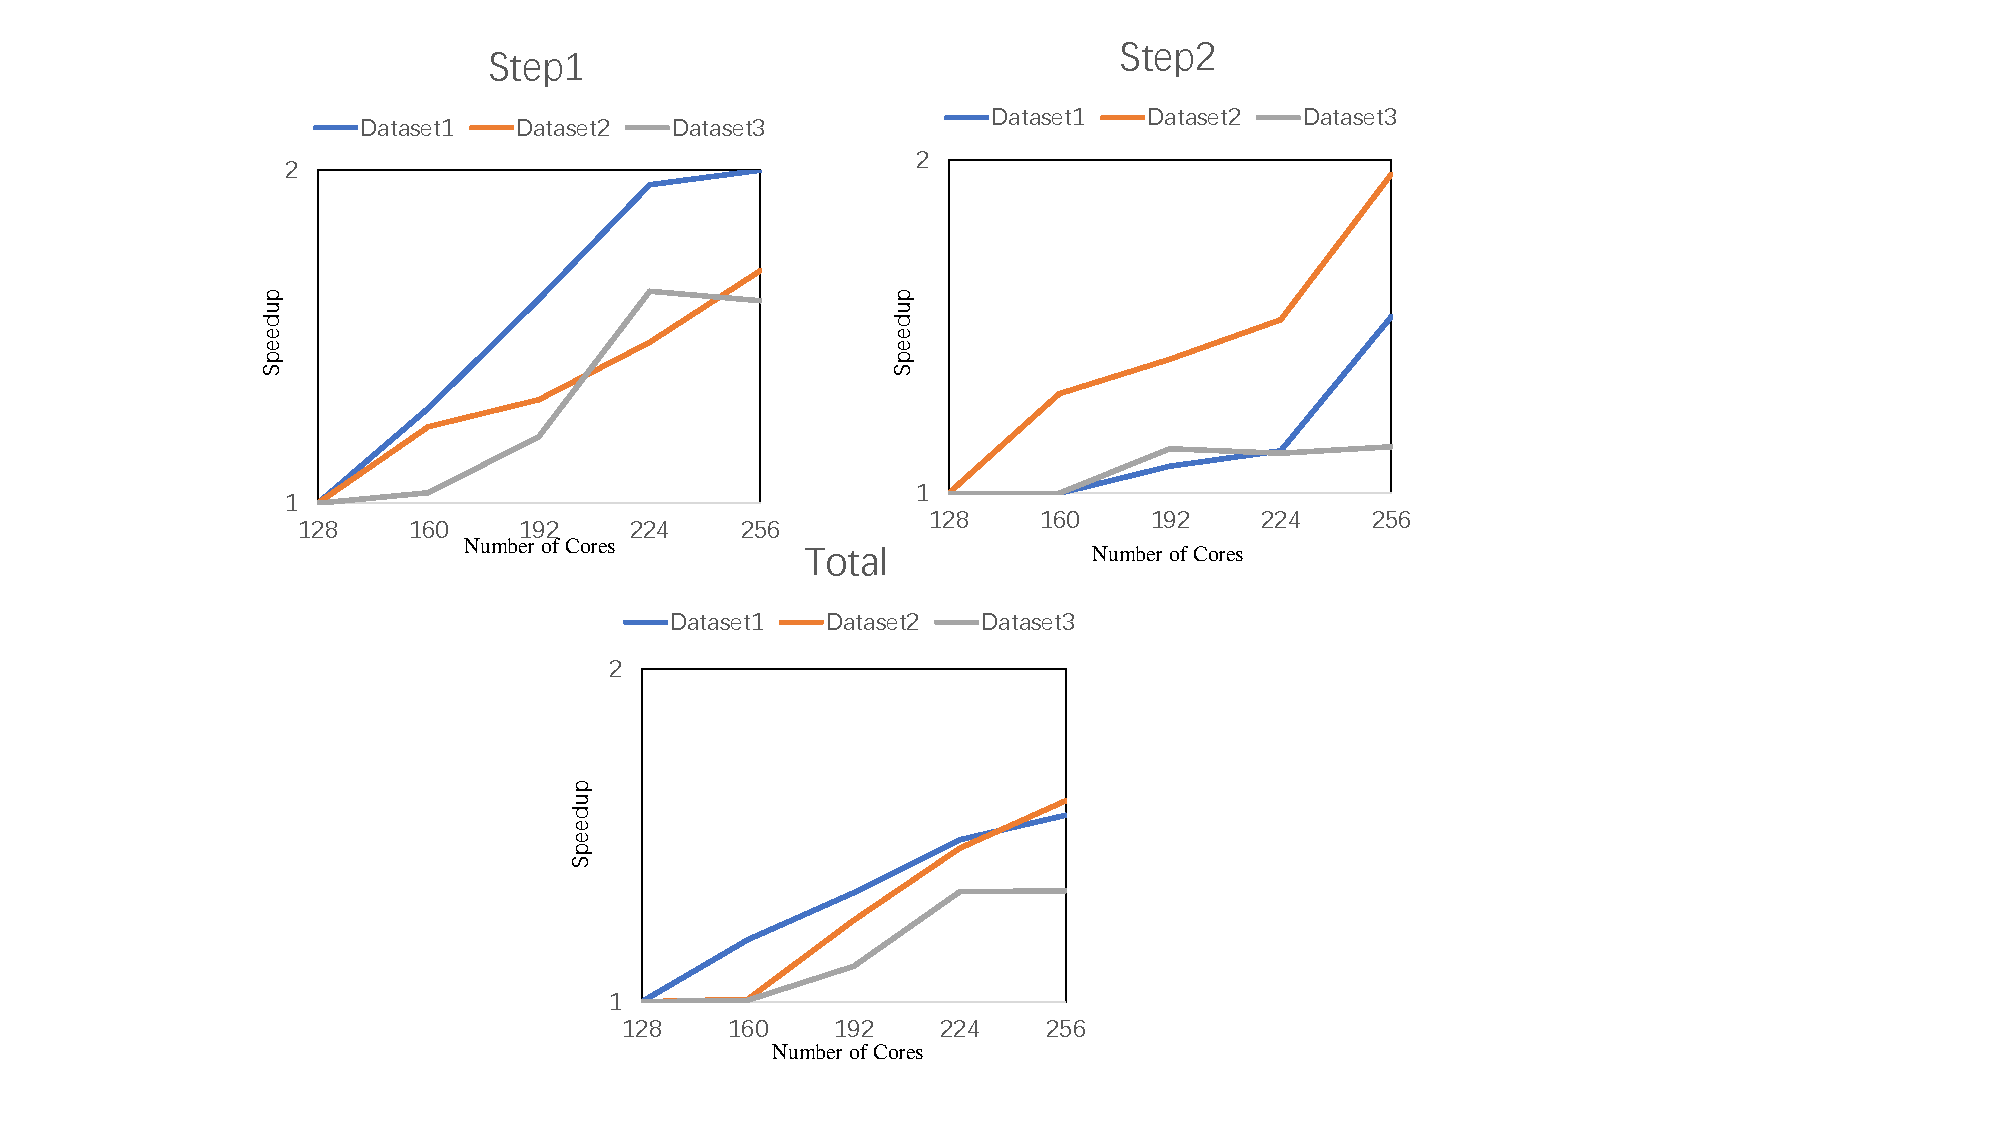
\includegraphics[width=0.45\textwidth]{fig5.pdf}
	\caption{An overview of pipelines' speedup.} \label{fig5}
\end{figure}
Due to the limited of single workstation CPU cores, we tested three tradition pipelines' speedup from 16 CPU cores to 64 CPU cores.
And due to the limited of memory capacity per node, we tested scSpark's speedup starting from 16 (1*16) CPU cores to 96 (6*16) CPU cores.

We found that UMI\-tools' performance can't take advantage of CPU core number increase because it only be supported on single\-thread mode except align step.
Although STAR can provides scalability on align step, the whole UMI\-tools pipeline's scalability is weak.
STAR-solo and Cellranger shows scalability when CPU cores number increase but will converage quickly.
When CPU cores number increased from 16 to 32, STAR-solo achieved approximate average 40\% speedup and Cellranger achieved approximate 10\% speedup.
When CPU cores number increased from 32 to 48, STAR-solo's speedup was average 30\% and Cellranger speedup was converage.
When CPU cores number increased from 48 to 60, STAR-solo's speedup was average xxx\%.

We found it can achieve average 50\% speedup when Spark's CPU cores number increased from 128 to 256.
So scSpark shows more scalability than three tradition pipelines when CPU cores number increase.

% scSpark不同核心数不同步骤的表现
\iffalse
\begin{table}
	\centering
	\caption{STAR's mapping speed}\label{tab3}
	\resizebox{0.45\textwidth}{!} {
	\begin{tabular}{l | l | l | l | l | l | l}
		\hline
		Dataset & 2 cores & 4 cores & 8 cores & 16 cores & 32 cores & 64 cores \\
		\hline
		PBMC\_human & 120.97 & 242.08 & 449.09 & 772.13 & 1389.32 & 961.59 \\
		PBMC\_rat &  & 261.23 & 530.57 & 1089 & 1391.24 & 1347.35 \\
		PBMC\_monkey  & 38.7 & 76.38 & 170.01 & 325.85 & 512.59 & 828.99 \\
		\hline
	\end{tabular} }
\end{table}
\fi
\begin{figure}
	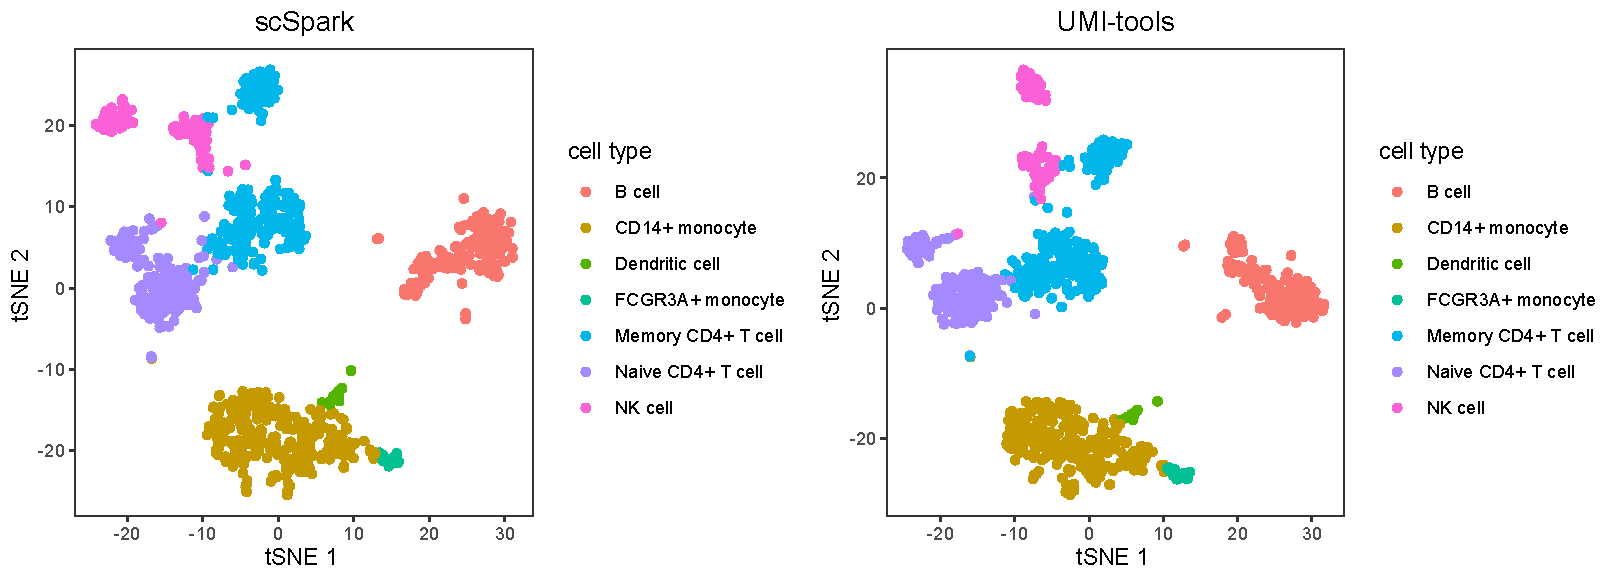
\includegraphics[width=0.45\textwidth]{fig7.pdf}
	\caption{scSpark's mapping speedup.} \label{fig7}
\end{figure}
As shown in Table~\ref{fig7}, we found in PBMC\_human and PBMC\_rat STAR can achieved nearly linear improved with CPU cores number increase, when CPU cores number below 32.
STAR's speedup rate not only decrease when CPU cores number increase but also have a bottleneck when CPU cores number increase from 32 to 64.
We found scSpark's mapping speed achieved about 79\% parallel efficiency when CPU cores number increase from 128 to 256.
ScSpark enable distributed process align step per node across Spark cluster, so it can get nearly linear parallel efficiency.
So scSpark's align step is more scalability than tradition pipelines' aligner. 

\subsection{Reliability of the results produced by scSpark} 
We further evaluated the accuracy of the expression matrices generated by scSpark.
First, the total UMI count for each cell in xxx dataset produced by scSpark was highly consistent with that by UMI-tools, with a Pearson correlation of $R^{2} = 0.9998$ (Fig~\ref{fig9}), which indicates that the expression profile of single cells produced by scSpark is reliable. In addition, we also evaluated whether scSpark would have influence on downstream biological analysis. Results show that the cell embeddings in tSNE map were highly consistent between scSpark and UMI-tools (Fig~\ref{fig10}). This further demonstrates that the expression matrices generated by scSpark are accurate and would not bring interference to various types of downstream analysis such as clustering, dimension reduction and cell type identification.
%As Fig~\ref{fig9} shown, for each after processing cell barcode, their gene expression matrix approximate fit $y=x$, $R^{2}$ closed to 0.9998. 
\begin{figure}
  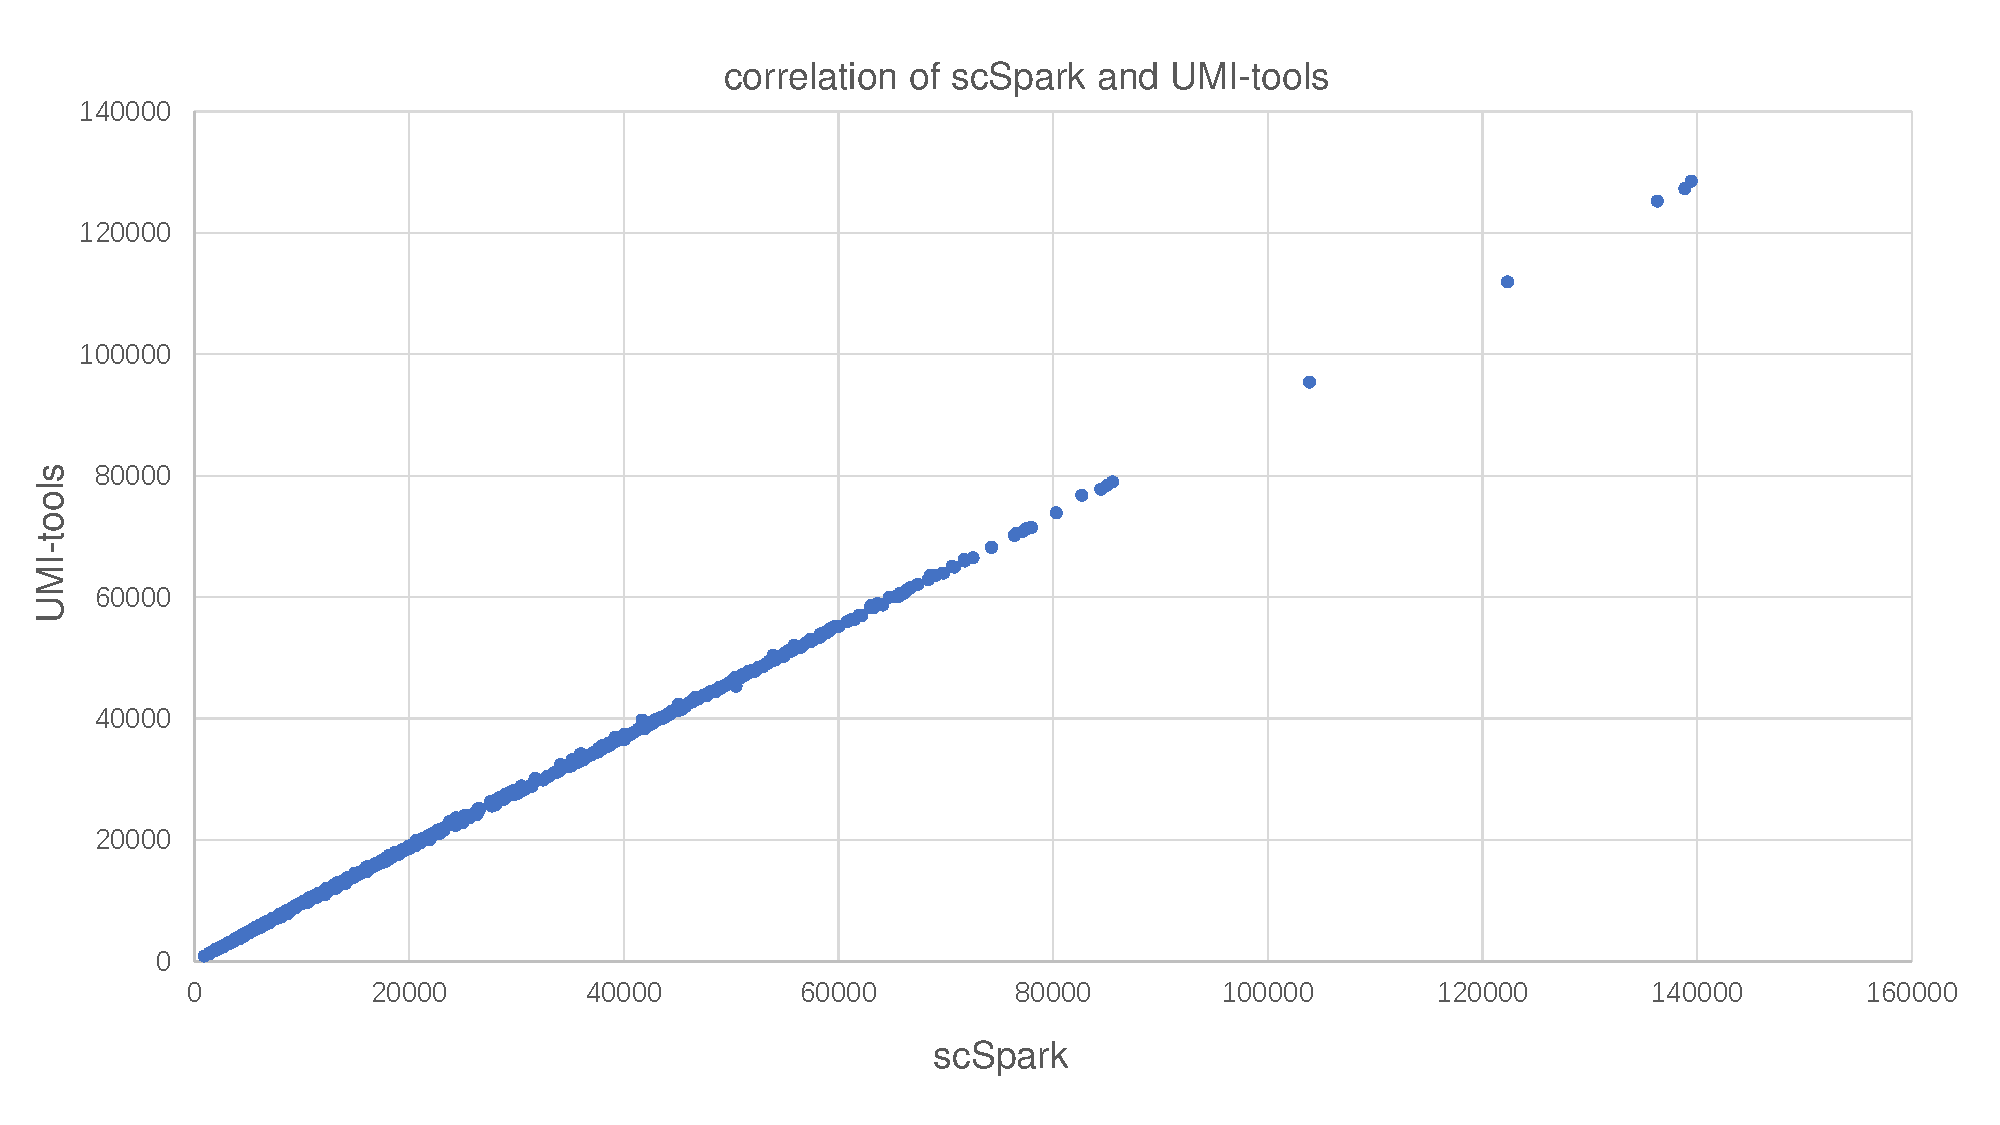
\includegraphics[width=0.45\textwidth]{fig9.pdf}
  \caption{correlation of scSpark and UMI-tools.} \label{fig9}
\end{figure}
%Furthermore, we used Seurat to print tSNE picture which based on gene expression matrix generated by ScSpark and UMI-tools. 
%And as Fig~\ref{fig10} shown, tSNE cell clustering result showed high corrleation between ScSpark and UMI-tools. 
\begin{figure*}
  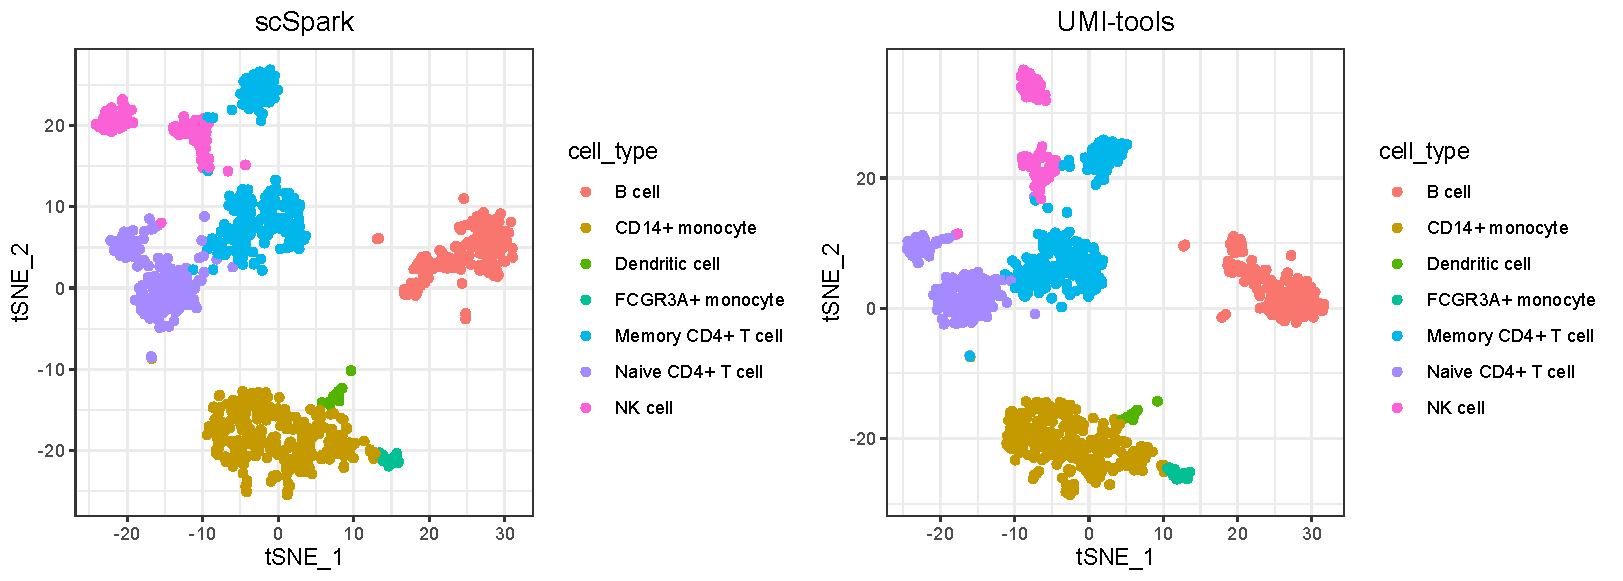
\includegraphics[width=\textwidth]{fig10.pdf}
  \caption{tSNE picture based on scSpark and UMI-tools' gene expression matrix.} \label{fig10}
\end{figure*}

\section{Conclusion}
% In this paper, we proposed a way which utilize Apache Spark's in-memory compute and distributed compute trait to strengthen upstream scRNA-seq pipeline.
% We developed scSpark, which processes more efficiency and more scalable than tradition pipelines.

% Refer to UMI-tools, scSpark divided the upstream process into four steps, UMI and CB correct, sequence quality control, genome alignment and transcript counting.
% we found scSpark's can get higher performance than three tradition pipelines.
% And we found scSpark's each steps can get higher performance than UMI-tools.
% We also compared scSpark's result with UMI-tools to verified scSpark's result correct.
To the volume and value of scRNA-seq data proliferated, we developed a pipeline scSpark.
ScSpark is an efficiently, highly scalable parallel compute pipeline on the top of Spark.
ScSpark not only more efficiently than tradition pipelines in same CPU cores number condition but also more scalability than tradition pipelines.
ScSpark's strategy reduce the exection time with speedup between 5 and 20 times at 64 CPU cores.
And scSpark can scale-out more than 256 CPU cores contrast with tradition pipelines' performance will converage when workstation scale-out 64 CPU cores.
We also believe that scSpark result biological was confirmed. 

\bibliographystyle{IEEEtran}
\bibliography{reference}

\end{document}
